% Chapter 8: S1S, the Büchi Theorem, and Deterministic Büchi Automata
% Sources: Course 89, L04 (att. 1129), L05 (att. 1130), L06 (att. 1131)

\chapter{S1S, the Büchi Theorem, and Deterministic Büchi Automata}
\label{ch:s1s-buchi}

The previous chapter introduced model checking as the central technique for
verifying reactive systems.  But what, mathematically, are we allowed to
\emph{say} about an infinite execution?  This chapter answers that question
by studying the \emph{Monadic Second-Order Theory of One Successor} (S1S),
a fragment of arithmetic powerful enough to express every $\omega$-regular
property, yet still decidable.

We will prove the landmark \textbf{Büchi Theorem} (1960): S1S and
non-deterministic Büchi automata are two different faces of the same
mathematical object---$\omega$-regular languages.  As a consequence,
the truth of any S1S sentence is decidable by an algorithm.  We will
also characterise the \emph{limits} of deterministic Büchi automata,
which turn out to be strictly weaker than their non-deterministic
counterparts---a fact that motivates the whole machinery of
complementation and, ultimately, the need for richer acceptance
conditions (Muller automata, studied in Chapter~\ref{ch:deterministic-automata-star-free}).

The chapter has one narrative spine.  First we learn how S1S talks about
positions of an infinite execution.  Then we turn formulas with free set
variables into $\omega$-words over bit-vectors.  That encoding lets every
logical operation become an automata operation: Boolean connectives become
closure constructions, and existential set quantification becomes
projection.  The Büchi theorem is the point where these translations meet.
The final section on deterministic Büchi automata is a deliberate bridge:
it keeps the theorem in view while explaining why the next chapter must
enrich deterministic acceptance conditions rather than merely repeat the
non-deterministic story.

% -----------------------------------------------------------------------
\section{The Time-Flow Perspective}
\label{sec:s1s-motivation}

A reactive system produces an infinite sequence of states
$s_0, s_1, s_2, \ldots$.  The indices $0, 1, 2, \ldots$ are just the
\emph{natural numbers $\mathbb{N}$}: the set of positions of an
$\omega$-word.  Every property we want to assert about the system is
therefore a property of $\mathbb{N}$ equipped with its successor function.

This is not an accident.  Historically, Büchi introduced non-deterministic
automata over infinite words precisely in order to prove that a certain
fragment of arithmetic---a logic about $\mathbb{N}$---is \emph{decidable}.
The resulting theory has since become the theoretical foundation of
virtually every temporal logic used in model checking.

\medskip\noindent
\textbf{Preview.}  The two logics we will study in the next chapters---LTL
and CTL---are \emph{not} S1S.  They are strictly less expressive, on
purpose.  LTL corresponds precisely to the \emph{first-order} fragment of
S1S (without second-order quantification).  Sacrificing second-order
quantification reduces decidability from \emph{non-elementary} complexity
to \emph{PSPACE-complete} for LTL and \emph{polynomial} for CTL---a
trade-off that makes model checking tractable in practice.  Understanding
S1S is therefore not merely academic: it is the bedrock on which the
whole temporal-logic edifice is built.

% -----------------------------------------------------------------------
\section{The Logic S1S}
\label{sec:s1s-def}

\subsection{Simple example: every \texorpdfstring{$a$}{a} is followed by a \texorpdfstring{$b$}{b}}
\label{sec:s1s-ex1}

\begin{example}
Let $A = \{a, b, c\}$.  Define the language:
\[
  L_1 = \{\alpha \in A^\omega \mid
          \text{every occurrence of } a \text{ is followed by some } b\}.
\]
An S1S$_A$ sentence for $L_1$:
\[
  \forall x.\; (x \in Q_a) \to (\exists y.\; x < y \land y \in Q_b).
\]
Reading in natural language: ``for every position $x$, if $a$ holds at
$x$, then there exists a future position $y > x$ where $b$ holds.''
\end{example}

Note how naturally the logic captures the English description: every
universal quantifier over positions $\forall x$ corresponds to ``for
every time point'', the predicate $Q_a$ says ``the symbol at that
position is $a$'', and $\exists y.\; x < y$ means ``there is a future
time point $y$''.

The time-flow perspective gives us the intended structure:
$0,1,2,\ldots$ with a successor operation.  S1S is the formal language for
talking about that structure.  First-order variables name individual time
positions; second-order variables name sets of positions, such as ``all
times where a request is pending''.

\subsection{S1S$_A$: S1S over an alphabet}

Let $A$ be a finite alphabet (a finite set of symbols).  We first define
\emph{S1S$_A$}, a version of the logic tailored to reason about
$\omega$-words over $A$.

\paragraph{Terms.}
Terms are built from:
\begin{itemize}
  \item the constant $0$ (zero);
  \item \emph{first-order variables} $x, y, z, \ldots$ (ranging over
        natural numbers, i.e., positions in a word); and
  \item the \emph{successor function} $+1$, applied to any term.
\end{itemize}
So $0$, $x$, $x+1$, $y+1+1$, etc.\ are all terms.  There is no subtraction
and no multiplication---these are the key restrictions that keep the logic
decidable.

\paragraph{Atomic formulas.}
An atomic formula has one of four forms:
\begin{enumerate}
  \item $t_1 = t_2$ \quad (equality between terms)
  \item $t_1 < t_2$ \quad (ordering: term $t_1$ is less than term $t_2$)
  \item $t \in X$ \quad (set membership: position $t$ belongs to the
        \emph{second-order variable} $X$, which ranges over \emph{sets} of
        natural numbers)
  \item $t \in Q_a$ \quad for each symbol $a \in A$ (the position $t$ is
        labelled by $a$ in the word being described)
\end{enumerate}

The predicates $Q_a$ are the interface between the logic and the words: they
``read'' the word at a given position.

\paragraph{Formulas.}
Full formulas are built from atomic formulas by:
\begin{itemize}
  \item Boolean connectives: $\neg$, $\land$, $\lor$, $\to$, $\leftrightarrow$;
  \item \emph{first-order} quantifiers: $\exists x$, $\forall x$ (over positions);
  \item \emph{second-order} quantifiers: $\exists X$, $\forall X$ (over
        sets of positions).
\end{itemize}
First-order variables are written as lowercase $x, y, z$; second-order
variables as uppercase $X, Y, Z$.

\begin{definition}[S1S$_A$ sentence]
A \emph{sentence} of S1S$_A$ is a formula with no free variables.  A
sentence has no parameters: it is either \emph{true} or \emph{false}
over a given structure, with no room for ambiguity about the value of
any variable.
\end{definition}

\subsection{Semantics: words as structures}

The key insight is to interpret an $\omega$-word $\alpha \in A^\omega$
as a mathematical \emph{structure}.

\begin{definition}[Word structure]
\label{def:word-structure}
Let $\alpha \in A^\omega$.  The \emph{word structure} $\overline{\alpha}$
is the tuple
\[
  \overline{\alpha} = \bigl(\mathbb{N},\; 0,\; {+1},\; {<},\;
                             \{Q_a\}_{a \in A}\bigr)
\]
where:
\begin{itemize}
  \item the domain is $\mathbb{N} = \{0, 1, 2, \ldots\}$;
  \item $0$, ${+1}$, and ${<}$ have their standard arithmetic meanings;
  \item $Q_a = \{i \in \mathbb{N} \mid \alpha(i) = a\}$ is the set of
        positions at which symbol $a$ appears in $\alpha$.
\end{itemize}
\end{definition}

\begin{example}[$Q_a$ for a periodic word]
Let $A = \{a, b\}$ and $\alpha = (ab)^\omega = ababab\cdots$.  Then:
\[
  Q_a = \{0, 2, 4, 6, \ldots\} = \text{even positions}, \qquad
  Q_b = \{1, 3, 5, 7, \ldots\} = \text{odd positions}.
\]
\end{example}

\begin{definition}[Language of a formula]
The \emph{language} of an S1S$_A$ sentence $\Phi$, written $L(\Phi)$,
is the set of all $\omega$-words $\alpha$ such that $\overline{\alpha}
\models \Phi$.
\end{definition}

This is exactly the notion of language we know from Büchi automata---a
set of $\omega$-words---but now defined logically.

% -----------------------------------------------------------------------
\section{What S1S Can Express}
\label{sec:s1s-expressive}

Before proving the Büchi theorem, let us develop an intuition for the
expressive power of S1S$_A$ through four examples of increasing
difficulty.  These patterns appear constantly in exam problems.
They also foreshadow the proof: every example below isolates a logical move
that later becomes an automata construction.



\subsection{Defining \texorpdfstring{$x < y$}{x < y} using only \texorpdfstring{$+1$}{+1}}
\label{sec:s1s-ordering}

The structure $\overline{\alpha}$ includes the ordering $<$, but it is
instructive to see that $<$ can actually be \emph{defined} using only
the successor function $+1$ and second-order variables---which shows
the power of the monadic quantification.

\begin{example}[Defining the ordering from the successor]
\label{ex:s1s-order}
We want to write a formula $\varphi(x, y)$ with two free variables that
holds if and only if $x < y$, using no occurrence of $<$.

\medskip\noindent
\textbf{Key idea.}  The set $\{x+1, x+2, x+3, \ldots\}$ is the
\emph{smallest} set that (a) contains $x+1$, and (b) is closed under
$+1$.  If $y$ is in this set, then $y > x$.

\medskip\noindent
\textbf{Wrong first attempt} (using $\exists X$):
\[
  \exists X.\;\bigl[(x+1) \in X \;\land\;
              \forall z.\; z \in X \to (z+1) \in X \;\land\;
              y \in X\bigr].
\]
This looks right, but is \emph{wrong}.  The problem: if $y < x$, we can
still choose $X = \mathbb{N}$, which satisfies all the conditions (it
contains $x+1$, is closed under $+1$, and contains $y$).  The existential
is too weak---it lets us pick any set, including ones that are ``too big''.

\textbf{Correcting the Existential Attempt}:
We \emph{can} make the existential definition work by adding a "breakpoint". We need to force the set $X$ to start strictly after $x$. We do this by simply forbidding $x \in X$:
\[
  \exists X.\;\bigl[x \notin X \;\land\; (x+1) \in X \;\land\;
              \forall z.\; z \in X \to (z+1) \in X \;\land\;
              y \in X\bigr].
\]
This prevents the choice of $X = \mathbb{N}$ and forces $X$ to be exactly $\{x+1, x+2, \ldots\}$ (or a subset of it, but closure under $+1$ makes it exactly that set).

\begin{center}
  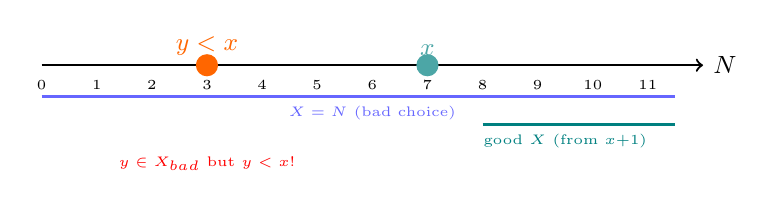
\begin{tikzpicture}[x=0.7cm, y=0.5cm]
    \draw[->, thick] (0,0) -- (12,0)
          node[right, font=\small] {$\mathbb{N}$};
    \foreach \i in {0,...,11}
      \node[font=\tiny, below=2pt] at (\i, 0) {$\i$};
    \fill[teal!70] (7,0) circle (4pt) node[above, font=\small]{$x$};
    \fill[orange!80!red] (3,0) circle (4pt) node[above, font=\small]{$y < x$};
    \draw[blue!60, very thick] (0, -0.8) -- (11.5, -0.8);
    \node[font=\tiny, blue!60, below] at (6, -0.8) {$X = \mathbb{N}$ (bad choice)};
    \draw[teal, very thick] (8, -1.5) -- (11.5, -1.5);
    \node[font=\tiny, teal, below] at (9.5, -1.5) {good $X$ (from $x{+}1$)};
    \node[font=\tiny, red] at (3, -2.5) {$y \in X_{\text{bad}}$ but $y < x$!};
  \end{tikzpicture}\par
  {\small\itshape With $\exists X$, one can always choose $X = \mathbb{N}$
  (blue), which contains both $x+1$ and $y$ even when $y < x$.}
\end{center}

\medskip\noindent
\textbf{Correct formula} (using $\forall X$):
\[
  \varphi(x, y) \;\equiv\;
  \forall X.\;\bigl[(x+1) \in X \;\land\;
                \forall z.\; z \in X \to (z+1) \in X\bigr]
             \to y \in X.
\]
Reading: ``for \emph{every} set $X$ that contains $x+1$ and is closed
under $+1$, $y$ must belong to $X$.''  Since the smallest such $X$ is
$\{x+1, x+2, \ldots\}$, and this set does \emph{not} contain any
$y \leq x$, the formula holds if and only if $y > x$.

Why does the wrong case fail now?  If $y < x$, take $X = \{x+1, x+2, \ldots\}$
(the \emph{minimal} candidate).  This set satisfies the hypothesis (contains
$x+1$ and is closed under $+1$), but does \emph{not} contain $y$.  So the
implication is false, and $\varphi(x, y)$ is false.  Correctness achieved.
\end{example}

\begin{remark}[Second-order universals are essential here]
The ordering $<$ is \emph{not} definable from $+1$ in the
\emph{first-order} fragment of S1S (without second-order quantifiers).
The inductive construction above fundamentally relies on the ability to
quantify over the \emph{set} of all successors, which is a second-order
concept.  This separation will reappear when we compare LTL to S1S.

However, the converse is true: we \emph{can} define the successor $+1$ from the ordering $<$ in purely first-order logic. The successor of $x$ is the strictly greater element $y$ such that there is no other element $z$ strictly between them:
\[
  y = x+1 \;\iff\; x < y \;\land\; \neg\exists z.\; (x < z \land z < y).
\]
\end{remark}

\subsection{Parity: positions of A in even locations}
\label{sec:s1s-parity}

\begin{example}[Even-position predicate]
\label{ex:s1s-parity}
Let $A = \{a, b\}$.  The language:
\[
  L_2 = \{\alpha \in A^\omega \mid \exists
          \text{ an even position } i \text{ with } \alpha(i) = a\}.
\]
First, we define a formula $\mathrm{Even}(y)$ asserting that $y$ is even.
The idea: the set of even numbers is the \emph{unique} set $X$ satisfying:
\begin{itemize}
  \item Base case: $0 \in X$.
  \item Alternating step: $\forall z.\; z \in X \leftrightarrow (z+1) \notin X$.
\end{itemize}
Note that the $\leftrightarrow$ (if-and-only-if) forces a strict alternation:
for every $z$ that is in $X$, its successor is \emph{not} in $X$, and vice
versa.  This produces exactly the set $\{0, 2, 4, 6, \ldots\}$.

\begin{center}
  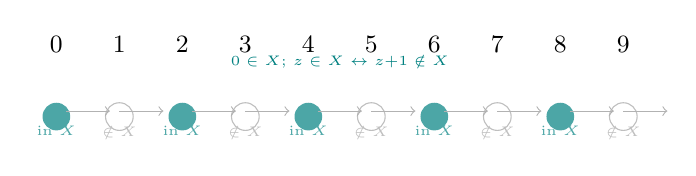
\begin{tikzpicture}[x=0.8cm, y=0.7cm]
    \foreach \i in {0,...,9}
      \node[font=\small] at (\i, 1.3) {\i};
    \foreach \i in {0,2,4,6,8}
      \fill[teal!70] (\i, 0) circle (5pt) node[below, font=\tiny]{in $X$};
    \foreach \i in {1,3,5,7,9}
      \draw[gray!50] (\i, 0) circle (5pt) node[below, font=\tiny]{$\notin X$};
    \foreach \i in {0,2,4,6,8} {
      \draw[->, gray!60, thin] (\i+0.15, 0.1) -- (\i+0.85, 0.1);
      \draw[->, gray!60, thin] (\i+0.85+0.15, 0.1) -- (\i+0.85+0.85, 0.1);
    }
    \node[font=\tiny, above, teal] at (4.5, 0.7)
          {$0 \in X$; $z \in X \leftrightarrow z{+}1 \notin X$};
  \end{tikzpicture}\par
  {\small\itshape Alternating definition of parity: starting from
  $0 \in X$, every even position is inside and every odd one outside.}
\end{center}

Because the set is uniquely determined by these constraints, existential and
universal quantification collapse: ``there exists an $X$ with these
properties'' and ``for all $X$ with these properties'' give the same answer.
The formula for $L_2$:
\begin{align*}
  \exists y.\; &(y \in Q_a) \;\land\\
               &\exists X.\;\bigl[0 \in X \;\land\;
                 \forall z.\; (z \in X \leftrightarrow (z+1) \notin X)\bigr]
               \;\land\; y \in X.
\end{align*}
\end{example}

\begin{remark}[Parity is not first-order]
The parity property is a canonical example of a property that is
\emph{not} expressible in the first-order fragment of S1S.  Its formula
makes essential use of a second-order variable $X$ to simulate induction.
This is directly connected to the fact that LTL cannot express ``$a$ occurs
at an even position''---temporal operators correspond to first-order
quantifiers, which are not powerful enough for parity.
\end{remark}

\subsection{Counting between consecutive occurrences}
\label{sec:s1s-counting}

\begin{example}[Even number of symbols between consecutive A's]
\label{ex:s1s-consecutive}
Let $A = \{a, b, c\}$.  Define:
\[
  L_3 = \{\alpha \in A^\omega \mid \text{between every pair of
          consecutive $a$'s, there is an even number of $b$'s or $c$'s}\}.
\]
(This is the same language for which we built a Büchi automaton in
Part~I.)  The S1S sentence proceeds in two parts:

\medskip\noindent
\textbf{Part 1: ``$x$ and $y$ are consecutive $a$'s.''} Positions $x$ and
$y$ are consecutive occurrences of $a$ if: $x \in Q_a$, $y \in Q_a$,
$x < y$, and there is no $z$ with $x < z < y$ and $z \in Q_a$:
\[
  \mathrm{consec}(x, y) \;\equiv\;
  x \in Q_a \;\land\; y \in Q_a \;\land\; x < y
  \;\land\; \neg\exists z.\;(x < z \land z < y \land z \in Q_a).
\]

\textbf{Part 2: ``$x$ and $y$ have the same parity.''} Using an alternating
set $X$ starting at $x$ (analogous to the parity example, but rooted at $x$):
\[
  \mathrm{sameParity}(x, y) \;\equiv\;
  \exists X.\;\bigl[x \in X \;\land\;
    \forall z.\;(z \in X \leftrightarrow (z+1) \notin X)\bigr]
  \;\land\; y \in X.
\]
If $y = x + 2k$ (even gap), they have the same parity; if $y = x + 2k+1$
(odd gap), different parity.  So ``even number of symbols in $(x, y)$''
means $y - x$ is even, which is exactly $\mathrm{sameParity}(x, y)$.

The full S1S sentence:
\[
  \forall x, y.\;
  \mathrm{consec}(x, y) \to \mathrm{sameParity}(x, y).
\]
\end{example}

\subsection{The key pattern: infinitely many occurrences}
\label{sec:s1s-infinitely}

\begin{example}[Infinitely many $a$'s]
\label{ex:s1s-infmany}
The language $L_\infty = \{\alpha \in A^\omega \mid \alpha \text{ contains
infinitely many } a\text{'s}\}$ is expressed by:
\[
  \Phi_\infty \;\equiv\; \forall x.\;\exists y.\; x < y \;\land\; y \in Q_a.
\]
Reading: ``for every time point $x$, there is a future time point $y$
where $a$ holds.''  This forces $a$ to appear arbitrarily far in the
future---equivalently, infinitely often.

\medskip\noindent
\textbf{Why not} $\forall x.\;(x \in Q_a) \to \exists y.\;x < y \land y \in Q_a$?
That formula has a trivially true antecedent: if there are \emph{no} $a$'s
at all, then $x \in Q_a$ is always false and the implication holds vacuously.
So the word $b^\omega$ (no $a$'s anywhere) would satisfy that formula---which
is wrong.  The correct $\Phi_\infty$ has no conditional: it asserts that
\emph{regardless} of what symbol is at $x$, a future $a$ must exist.
\end{example}

\begin{figure}[ht]
  \centering
  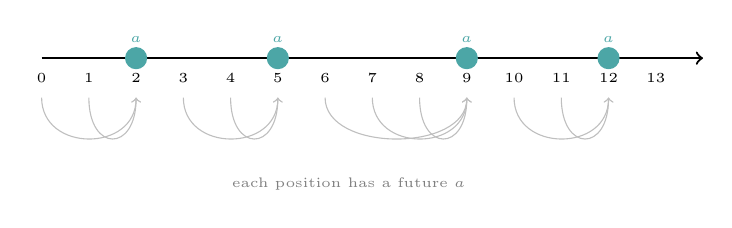
\begin{tikzpicture}[x=0.6cm]
    \draw[->, thick] (0,0) -- (14,0);
    \foreach \i in {0,...,13}
      \node[font=\tiny, below=2pt] at (\i, 0) {$\i$};
    % a's at positions 2,5,9,12
    \foreach \i in {2,5,9,12}
      \fill[teal!70] (\i,0) circle (4pt) node[above=2pt, font=\tiny]{$a$};
    % "for all x" arrows
    \foreach \x/\y in {0/2, 1/2, 3/5, 4/5, 6/9, 7/9, 8/9, 10/12, 11/12} {
      \draw[->, gray!50, thin]
            (\x, -0.5) .. controls (\x, -1.2) and (\y, -1.2) .. (\y, -0.5);
    }
    \node[font=\tiny, gray] at (6.5,-1.6)
          {each position has a future $a$};
  \end{tikzpicture}
  \caption{The $\forall x\,\exists y$ pattern for ``infinitely many $a$'s''.
           Every position (including non-$a$ ones) has a future occurrence of
           $a$ to witness the existential.  This pattern is the S1S counterpart
           of the LTL operator $\mathbf{GF}\,a$ (``globally eventually $a$'').}
  \label{fig:s1s-infmany}
\end{figure}

\begin{remark}[$\forall x\,\exists y$ = $\mathbf{GF}$ in LTL]
The pattern $\forall x.\;\exists y.\;x < y \land P(y)$ is one of the most
recurring in S1S, model checking, and temporal logic.  In LTL it corresponds
to $\mathbf{G}(\mathbf{F}\,P)$ (``$P$ holds infinitely often'').  In fairness
constraints, the same infinitely-often pattern appears in NuSMV
\texttt{JUSTICE} clauses (Chapter~\ref{ch:reactive-smv}).
\end{remark}

% -----------------------------------------------------------------------
\section{Free Variables and the Encoding \texorpdfstring{$\{0,1\}^n$}{0-1-n}}
\label{sec:s1s-encoding}

So far we have treated S1S$_A$ for sentences (no free variables).  For the
Büchi theorem proof, we need to handle \emph{open formulas} with $n$ free
\emph{second-order} variables $X_1, \ldots, X_n$.
This is not just a technical detail: it is the mechanism that lets logic
and automata communicate.  An automaton reads a word, so a valuation for the
free variables must itself be presented as a word.

\subsection{Why free variables complicate things}

A sentence $\Phi$ is true or false over $\overline{\alpha}$---there are
no parameters.  But a formula $\Psi(X_1, X_2)$ with two free SO variables
needs an \emph{interpretation} of $X_1$ and $X_2$ (as sets of naturals)
before it can be evaluated.  A single $\omega$-word does not carry this
information.

\subsection{Words as value assignments}

The elegant solution: \emph{encode} the value of all free variables
inside the word itself.  Instead of words over $A$, use words over
$\{0,1\}^n$, where each position carries an $n$-bit tuple that specifies,
for each variable $X_k$, whether that position belongs to $X_k$.

\begin{definition}[Free-variable encoding]
Given a formula $\Phi(X_1, \ldots, X_n)$ with $n$ free SO variables and
an $\omega$-word $\alpha \in (\{0,1\}^n)^\omega$, define:
\[
  P_k = \{i \in \mathbb{N} \mid \alpha(i)_k = 1\}
\]
where $\alpha(i)_k$ is the $k$-th bit of the $n$-tuple at position $i$.
The set $P_k$ is the \emph{interpretation} assigned to $X_k$ by the
word $\alpha$.
\end{definition}

\begin{example}[Visualising the encoding]
Suppose $n = 2$ (variables $X_1$, $X_2$) and the word is:
\[
  \alpha = \underbrace{\binom{1}{1}}_{\alpha(0)}\;
           \underbrace{\binom{0}{1}}_{\alpha(1)}\;
           \underbrace{\binom{1}{0}}_{\alpha(2)}\;
           \underbrace{\binom{0}{0}}_{\alpha(3)}\;
           \underbrace{\binom{1}{0}}_{\alpha(4)}\;\cdots
\]
Reading by rows: row 1 (top) encodes $X_1$; row 2 (bottom) encodes $X_2$.
\[
  X_1 = P_1 = \{0, 2, 4, \ldots\}, \qquad
  X_2 = P_2 = \{0, 1\}.
\]
So this word represents the interpretation ``$X_1$ is the set of even
numbers; $X_2$ is the set $\{0,1\}$''.
\end{example}

\begin{figure}[ht]
  \centering
  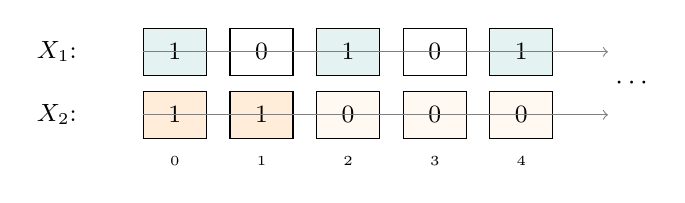
\begin{tikzpicture}
    \node[font=\small] at (-1.5, 0.5) {$X_1$:};
    \node[font=\small] at (-1.5, -0.3) {$X_2$:};
    \foreach \i/\a/\b in {0/1/1, 1/0/1, 2/1/0, 3/0/0, 4/1/0} {
      \node[font=\small, minimum width=0.8cm, minimum height=0.6cm,
            draw, fill=teal!\a0!white] at (\i*1.1, 0.5) {\a};
      \node[font=\small, minimum width=0.8cm, minimum height=0.6cm,
            draw, fill=orange!\b5!white] at (\i*1.1, -0.3) {\b};
      \node[font=\tiny, below=3pt] at (\i*1.1, -0.6) {$\i$};
    }
    \node at (5.8, 0.1) {$\cdots$};
    \draw[->, gray] (-0.4, 0.5) -- (5.5, 0.5);
    \draw[->, gray] (-0.4, -0.3) -- (5.5, -0.3);
  \end{tikzpicture}
  \caption{Encoding two free SO variables $X_1$ (top row, teal) and $X_2$
           (bottom row, orange) as an $\omega$-word over $\{0,1\}^2$.
           Each column is one position; a~$1$ means ``this position belongs
           to the variable''.  The word uniquely determines the interpretation
           $X_1 = \{0,2,4,\ldots\}$ and $X_2 = \{0,1\}$.}
  \label{fig:s1s-encoding}
\end{figure}

This encoding is key: a formula with $n$ free SO variables becomes a
\emph{language} over $\{0,1\}^n$.  Every closure property (union,
intersection, complementation, projection) for Büchi automata over
$\{0,1\}^n$ then translates directly to a logical operation on formulas.

\paragraph{S1S$_A \equiv$ S1S.}
S1S$_A$ (with alphabet predicates $Q_a$) can be converted to S1S (pure
arithmetic, no alphabet) by replacing each symbol $a \in A$ with a binary
encoding of length $\lceil \log_2 |A| \rceil$.  The two logics are
expressively equivalent; we use whichever is more convenient.

% -----------------------------------------------------------------------
\section{The Büchi Theorem}
\label{sec:buchi-theorem}

At this point the two sides have the same shape.  An S1S sentence defines a
set of infinite words; a Büchi automaton recognises a set of infinite words.
The theorem says that these two ways of describing sets are extensionally
identical.

We can now state the central result.

\begin{theorem}[Büchi, 1960]
\label{thm:buchi}
An $\omega$-language $L \subseteq A^\omega$ is \emph{$\omega$-regular}
(recognised by some non-deterministic Büchi automaton) if and only if it
is \emph{S1S-definable} (equal to $L(\Phi)$ for some S1S$_A$ sentence
$\Phi$).
\end{theorem}

Both directions are constructive: the proofs give explicit algorithms for
translating between automata and formulas.  Before the proof, note what
this theorem means:

\begin{itemize}
  \item \textbf{Declarative $\leftrightarrow$ Operational.}  S1S is a
        \emph{declarative} language (describe what you want); Büchi automata
        are \emph{operational} (describe how to process a word step by step).
        The theorem says they define exactly the same class of languages.
  \item \textbf{Succintness.}  S1S can be exponentially more succinct
        than Büchi automata: there exist S1S sentences of size $n$ whose
        smallest equivalent Büchi automaton has exponentially many states.
  \item \textbf{Decidability.}  The theorem implies that \emph{all} Büchi
        automaton operations (emptiness, inclusion, etc.) have logical
        counterparts, and vice versa.
\end{itemize}

% -----------------------------------------------------------------------
\section{Proof: \texorpdfstring{$\omega$-regular $\Rightarrow$ S1S-definable}{omega-regular implies S1S-definable}}
\label{sec:buchi-proof-fwd}

This is the easier direction.  An accepting run is already an infinite
object indexed by time; S1S only has to guess that run using sets of
positions and then check that the guessed run starts correctly, follows the
transition relation, and satisfies the Büchi condition.

\textbf{Given:} NBA $\mathcal{A} = (Q, A, \delta, q_0, F)$ with states
$Q = \{0, 1, \ldots, m\}$ (we name the initial state $0$).

\textbf{Goal:} Write an S1S sentence $\Phi_{\mathcal{A}}$ such that
$L(\Phi_{\mathcal{A}}) = L(\mathcal{A})$.

\subsection{The main idea: encode a run as a family of sets}

A run of $\mathcal{A}$ over a word $\alpha$ is an infinite sequence of
states $\sigma = q_{i_0} q_{i_1} q_{i_2} \cdots$.  We encode this run
using $m+1$ second-order variables $Y_0, \ldots, Y_m$, one per state:
\[
  Y_i = \{j \in \mathbb{N} \mid \sigma(j) = i\}
      = \text{``the set of positions where the run is in state } i\text{''}.
\]
If the run visits state 3 at positions 0, 4, 17, $\ldots$, then
$Y_3 = \{0, 4, 17, \ldots\}$.  The run is fully determined by the
partition $Y_0, \ldots, Y_m$ of $\mathbb{N}$.

Non-determinism is encoded by the \emph{choice} of these sets: different
choices of $Y_0, \ldots, Y_m$ correspond to different runs of the
(non-deterministic) automaton.

\subsection{The three conditions}

We write $\Phi_{\mathcal{A}} \equiv \exists Y_0 \cdots \exists Y_m.\;
\varphi_1 \land \varphi_2 \land \varphi_3$ where:

\paragraph{$\varphi_1$: Initiality.}
The run starts in state $q_0 = 0$ and the sets are pairwise disjoint
(the automaton is in exactly one state at each position):
\[
  \varphi_1 \;\equiv\;
  (0 \in Y_0) \;\land\;
  \bigwedge_{i \neq j}\; \neg\exists x.\;(x \in Y_i \land x \in Y_j).
\]

\paragraph{$\varphi_2$: Consequentiality.}
The run follows the transition relation: at each position $x$, if the
automaton is in state $i$ and reads symbol $a$, it moves to state $j$:
\[
  \varphi_2 \;\equiv\;
  \forall x.\;
  \bigvee_{(i,a,j) \in \delta}
    \bigl(x \in Y_i \;\land\; x \in Q_a \;\land\; (x+1) \in Y_j\bigr).
\]
Every position must be covered by exactly one transition.

\paragraph{$\varphi_3$: Acceptance.}
At least one final state is visited infinitely often (using the
$\forall x\,\exists y$ pattern from Example~\ref{ex:s1s-infmany}):
\[
  \varphi_3 \;\equiv\;
  \bigvee_{i \in F}\;
    \forall x.\;\exists y.\; x < y \;\land\; y \in Y_i.
\]

\begin{figure}[ht]
  \centering
  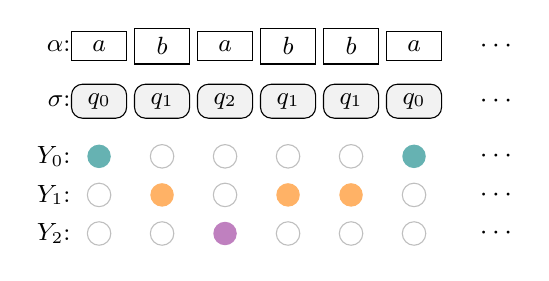
\begin{tikzpicture}[x=0.8cm, y=0.7cm]
    \node[left, font=\small] at (-0.3, 2.5) {$\alpha$:};
    \foreach \i/\sym in {0/a, 1/b, 2/a, 3/b, 4/b, 5/a} {
      \node[font=\small, draw, minimum width=0.7cm] at (\i, 2.5) {$\sym$};
    }
    \node at (6.3, 2.5) {$\cdots$};
    \node[left, font=\small] at (-0.3, 1.5) {$\sigma$:};
    \foreach \i/\st in {0/0, 1/1, 2/2, 3/1, 4/1, 5/0} {
      \node[font=\small, draw, rounded corners, minimum width=0.7cm, fill=gray!10]
            at (\i, 1.5) {$q_\st$};
    }
    \node at (6.3, 1.5) {$\cdots$};
    \node[left, font=\small] at (-0.3, 0.5) {$Y_0$:};
    \node[circle, inner sep=3pt, fill=teal!60]  at (0, 0.5) {};
    \node[circle, inner sep=3pt, draw=gray!50]  at (1, 0.5) {};
    \node[circle, inner sep=3pt, draw=gray!50]  at (2, 0.5) {};
    \node[circle, inner sep=3pt, draw=gray!50]  at (3, 0.5) {};
    \node[circle, inner sep=3pt, draw=gray!50]  at (4, 0.5) {};
    \node[circle, inner sep=3pt, fill=teal!60]  at (5, 0.5) {};
    \node at (6.3, 0.5) {$\cdots$};

    \node[left, font=\small] at (-0.3, -0.2) {$Y_1$:};
    \node[circle, inner sep=3pt, draw=gray!50]    at (0, -0.2) {};
    \node[circle, inner sep=3pt, fill=orange!60]  at (1, -0.2) {};
    \node[circle, inner sep=3pt, draw=gray!50]    at (2, -0.2) {};
    \node[circle, inner sep=3pt, fill=orange!60]  at (3, -0.2) {};
    \node[circle, inner sep=3pt, fill=orange!60]  at (4, -0.2) {};
    \node[circle, inner sep=3pt, draw=gray!50]    at (5, -0.2) {};
    \node at (6.3, -0.2) {$\cdots$};

    \node[left, font=\small] at (-0.3, -0.9) {$Y_2$:};
    \node[circle, inner sep=3pt, draw=gray!50]    at (0, -0.9) {};
    \node[circle, inner sep=3pt, draw=gray!50]    at (1, -0.9) {};
    \node[circle, inner sep=3pt, fill=violet!50]  at (2, -0.9) {};
    \node[circle, inner sep=3pt, draw=gray!50]    at (3, -0.9) {};
    \node[circle, inner sep=3pt, draw=gray!50]    at (4, -0.9) {};
    \node[circle, inner sep=3pt, draw=gray!50]    at (5, -0.9) {};
    \node at (6.3, -0.9) {$\cdots$};
  \end{tikzpicture}
  \caption{Encoding a run $\sigma = q_0 q_1 q_2 q_1 q_1 q_0 \cdots$ of
           a 3-state automaton as sets $Y_0$ (teal), $Y_1$ (orange),
           $Y_2$ (violet).  At each position exactly one set contains a
           filled dot.  This encoding converts the run into an
           interpretation of the S1S second-order variables.}
  \label{fig:s1s-run-encoding}
\end{figure}

\begin{theorem}[Correctness]
$\overline{\alpha} \models \Phi_{\mathcal{A}}$ if and only if
$\alpha \in L(\mathcal{A})$.
\end{theorem}
\begin{proof}[Proof sketch]
($\Rightarrow$) If $\overline{\alpha} \models \Phi_{\mathcal{A}}$, then
the existential witnesses $Y_0, \ldots, Y_m$ define a run of $\mathcal{A}$
over $\alpha$ ($\varphi_1$ gives initiality, $\varphi_2$ gives valid
transitions, $\varphi_3$ gives acceptance).  Hence $\alpha \in
L(\mathcal{A})$.  ($\Leftarrow$) If $\alpha \in L(\mathcal{A})$, there
exists an accepting run $\sigma$.  Setting $Y_i = \{j \mid \sigma(j) = i\}$
satisfies all three conditions.
\end{proof}

% -----------------------------------------------------------------------
\section{Closure under Projection}
\label{sec:closure-projection}

Before proving the other direction of the Büchi theorem, we need one more
closure property of Büchi automata: \emph{closure under projection}.  This
corresponds, logically, to \emph{existential second-order quantification}.
This is the central bridge from syntax to automata: forgetting one bit of
the input word is the automata-theoretic version of saying ``there exists a
set of positions with this property''.

\begin{lemma}[Closure under projection]
\label{lem:projection}
Let $\mathcal{A}$ be an NBA over $\{0,1\}^n$ recognising $L(\Phi)$,
where $\Phi$ has $n$ free SO variables.  Let $\Psi \equiv \exists X_i.\;\Phi$
(with $n-1$ free variables).  Then there exists an NBA $\mathcal{A}'$ over
$\{0,1\}^{n-1}$ recognising $L(\Psi)$.
\end{lemma}

\begin{proof}[Construction]
$\mathcal{A}'$ is obtained from $\mathcal{A}$ by \emph{removing the
$i$-th bit from every transition label}.  If $\mathcal{A}$ has a
transition $q \xrightarrow{(b_1,\ldots,b_n)} q'$, then $\mathcal{A}'$
has a transition $q \xrightarrow{(b_1,\ldots,b_{i-1},b_{i+1},\ldots,b_n)} q'$.
\end{proof}

\medskip\noindent
\textbf{Intuition.}  Existential quantification over $X_i$ means: ``there
\emph{exists} a value for the $i$-th row of the word such that $\Phi$
holds.''  By removing the $i$-th bit from the alphabet, we allow the
automaton to process words of length $n-1$ and non-deterministically
``guess'' what the missing $i$-th bit could have been.

\begin{example}[Projection reduces the alphabet]
An NBA $\mathcal{A}$ over $\{0,1\}^2 = \{00, 01, 10, 11\}$ with transitions:
\[
  q_0 \xrightarrow{00} q_1, \quad
  q_1 \xrightarrow{11} q_1, \quad
  q_1 \xrightarrow{10} q_2, \quad
  q_2 \xrightarrow{11} q_2
\]
After projecting onto the first component (removing the second bit):
\[
  q_0 \xrightarrow{0} q_1, \quad
  q_1 \xrightarrow{1} q_1, \quad
  q_1 \xrightarrow{1} q_2, \quad
  q_2 \xrightarrow{1} q_2.
\]
The resulting $\mathcal{A}'$ over $\{0,1\}$ is \emph{non-deterministic}
(two transitions from $q_1$ on symbol $1$), because the second component
is now ``free'' to take any value.
\end{example}

% -----------------------------------------------------------------------
\section{Proof: S1S-definable \texorpdfstring{$\Rightarrow$}{=>} \texorpdfstring{$\omega$-regular}{omega-regular}}
\label{sec:buchi-proof-bwd}

This is the more involved direction: given an S1S formula, construct an
NBA.  The strategy is a two-step normalisation.
First we reduce the logic to a tiny kernel with only set variables and two
atomic predicates.  Then we show that this kernel has base automata and is
closed under the operations used to build formulas.

\subsection{Step 1: S1S $\to$ S1S$_0$ (syntactic simplification)}

S1S$_0$ is an extremely restricted fragment:
\begin{itemize}
  \item \textbf{Only second-order variables} (no first-order variables).
  \item \textbf{Only two atomic predicates}: $X \subseteq Y$ (subset
        relation) and $\mathrm{Succ}(X, Y)$ (``$X = \{x\}$, $Y = \{x+1\}$
        are consecutive singletons'').
  \item Boolean connectives and second-order quantifiers as usual.
\end{itemize}

Despite its extreme simplicity, S1S$_0$ is expressively equivalent to S1S.
The translation proceeds through four rewriting steps:

\paragraph{Step 1a: Isolate uses of $+1$.}
Rewrite every atomic formula so that $+1$ appears only in an equality:
``$x+1 = y$''.  For example, $x+1 \in X$ becomes $\exists y.\;(y = x+1)
\land (y \in X)$.  Nested successors introduce extra auxiliary variables:
$x+1+1 \in X$ becomes $\exists y.\,\exists z.\;y = x+1 \land z = y+1
\land z \in X$.

\paragraph{Step 1b: Remove the constant $0$ and the relation $<$.}
Using the definitions from Section~\ref{sec:s1s-ordering}:
$0$ is the unique position $x$ with no predecessor; $x < y$ is defined
by the $\forall X$ formula from Example~\ref{ex:s1s-order}.

\paragraph{Step 1c: Eliminate first-order variables.}
Replace every first-order variable $x$ with a second-order singleton
variable $X$ (a set containing exactly one element):
\begin{align*}
  \exists x.\;\varphi(x) &\quad\mapsto\quad \exists X.\;\mathrm{Singleton}(X) \land \varphi(X), \\
  \forall x.\;\varphi(x) &\quad\mapsto\quad \forall X.\;\mathrm{Singleton}(X) \to \varphi(X).
\end{align*}
Here $\mathrm{Singleton}(X)$ asserts $X$ has exactly one element. While we could define it using $\mathrm{Succ}(X,Y)$, we can construct it more cleanly using \emph{only} the subset relation $\subseteq$ by viewing sets as a lattice:
\[
  \mathrm{Singleton}(X) \;\equiv\;
  \exists Y \subseteq X.\; \bigl(Y \neq X \;\land\; \neg\exists Z.\; (Y \subseteq Z \land Z \subseteq X \land Z \neq Y \land Z \neq X)\bigr).
\]
Because $Y$ is a strict subset of $X$ with no sets strictly between them, $X$ can only have exactly one more element than $Y$. Furthermore, by forcing $Y$ to be the empty set (which we can define as $Y \subseteq W$ for all $W$), this completely constrains $X$ to have exactly one element.

\paragraph{Walkthrough: Reducing a formula to S1S$_0$}
Let's see this process in action at the whiteboard. Suppose we start with the simple property: ``the successor of position $x$ is labelled $a$'', which is written as $x+1 \in Q_a$.
\begin{enumerate}
    \item \textbf{Isolate $+1$}: We extract the successor into an equality.
          $\exists y.\; (y = x+1 \land y \in Q_a)$.
    \item \textbf{Eliminate FO variables}: We replace the positions $x$ and $y$ with singleton sets $X$ and $Y$.
          $\exists X.\; \mathrm{Singleton}(X) \land \exists Y.\; \mathrm{Singleton}(Y) \land \dots$
    \item \textbf{Rewrite atomics}: The equality $y = x+1$ becomes $\mathrm{Succ}(X, Y)$. The membership $y \in Q_a$ means the set $Y$ is a subset of the set of positions labelled $a$, which is just $Y \subseteq Q_a$.
\end{enumerate}
The final S1S$_0$ formula is:
\[
  \exists X.\, \exists Y.\; \mathrm{Singleton}(X) \land \mathrm{Singleton}(Y) \land \mathrm{Succ}(X, Y) \land Y \subseteq Q_a.
\]
This uses only second-order variables and the base predicates.

\paragraph{Step 1d: Rewrite remaining atomic formulas.}
After the above steps, every atomic formula has one of these forms,
which are directly expressible in S1S$_0$:
\begin{itemize}
  \item $X = Y$ $\;\equiv\;$ $X \subseteq Y \land Y \subseteq X$
  \item $X \neq Y$ $\;\equiv\;$ $\neg(X = Y)$
  \item $x+1 = y$ $\;\equiv\;$ $\mathrm{Succ}(\{x\}, \{y\})$
        (using the singleton encoding)
  \item $x \in X$ $\;\equiv\;$ $\{x\} \subseteq X$
\end{itemize}

\subsection{Step 2: S1S$_0$ $\to$ NBA (base cases and closure)}

With S1S$_0$ in hand, we build NBAs recursively on the formula structure:
\begin{itemize}
  \item \textbf{Boolean operators}: closure under union ($\lor$),
        intersection ($\land$), complementation ($\neg$).
  \item \textbf{Existential quantifier} $\exists X_i$: closure under
        projection (Lemma~\ref{lem:projection}).
\end{itemize}
It remains to give NBAs for the two atomic predicates of S1S$_0$.

\paragraph{Automaton for $X \subseteq Y$.}
This formula has two free SO variables, so the alphabet is $\{0,1\}^2$.
An $\omega$-word over $\{0,1\}^2$ encodes $X$ (first bit) and $Y$ (second
bit).  $X \subseteq Y$ holds iff every position where the first bit is 1
also has the second bit equal to 1---i.e., the symbol $(1,0)$ never occurs.

\begin{figure}[ht]
  \centering
  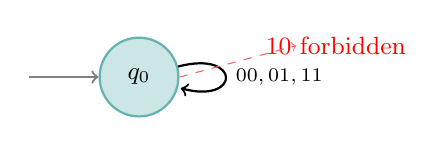
\begin{tikzpicture}[
    st/.style={draw, circle, minimum size=1cm, font=\small},
    arr/.style={->, thick}]
    \node[st, fill=teal!20, draw=teal!60, thick] (q0) at (0,0) {$q_0$};
    \draw[->, gray, thick] (-1.4, 0) -- (q0);
    \draw[arr] (q0) edge[loop right] node[right]
          {\scriptsize$00, 01, 11$} (q0);
    \node[red, font=\small] at (2.5, 0.4) {$10$ forbidden};
    \draw[->, red!60, dashed] (q0.east) -- (2.0, 0.4);
  \end{tikzpicture}
  \caption{NBA for $X \subseteq Y$ over $\{0,1\}^2$.  A single accepting
           state loops on all symbols except $(1,0)$ (which would mean
           ``position in $X$ but not in $Y$'', violating $X \subseteq Y$).
           Words containing $(1,0)$ have no accepting run.}
  \label{fig:nba-subset}
\end{figure}

\paragraph{Automaton for $\mathrm{Succ}(X, Y)$.}
This asserts: $X = \{x\}$, $Y = \{x+1\}$ for some $x$.  Three states suffice:

\begin{figure}[ht]
  \centering
  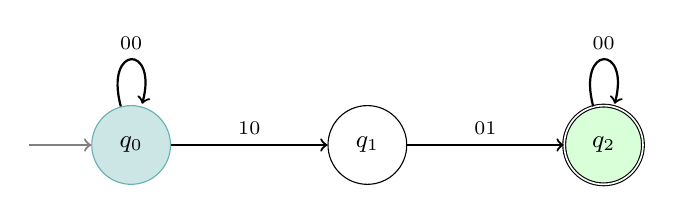
\begin{tikzpicture}[
    st/.style={draw, circle, minimum size=1cm, font=\small},
    acc/.style={draw, circle, minimum size=1cm, font=\small, double},
    arr/.style={->, thick}]
    \node[st, fill=teal!20, draw=teal!60] (q0) at (0,0) {$q_0$};
    \node[st] (q1) at (3,0) {$q_1$};
    \node[acc, fill=green!15] (q2) at (6,0) {$q_2$};
    \draw[->, gray, thick] (-1.3,0) -- (q0);
    \draw[arr] (q0) edge[loop above] node[above]{\scriptsize$00$} (q0);
    \draw[arr] (q0) -- node[above]{\scriptsize$10$} (q1);
    \draw[arr] (q1) -- node[above]{\scriptsize$01$} (q2);
    \draw[arr] (q2) edge[loop above] node[above]{\scriptsize$00$} (q2);
  \end{tikzpicture}
  \caption{NBA for $\mathrm{Succ}(X,Y)$ over $\{0,1\}^2$.  State $q_0$
           waits for the single $1$ in $X$ (symbol $10$: position in $X$,
           not yet in $Y$).  State $q_1$ sees the single $1$ in $Y$ (symbol
           $01$: position in $Y$, immediately after $X$'s element).  State
           $q_2$ (accepting) loops on $00$ forever.  Any other symbol causes
           a stuck run (no transition), rejecting the word.}
  \label{fig:nba-succ}
\end{figure}

With these two base automata and the closure properties, the recursive
construction of an NBA for any S1S$_0$ formula---and hence any S1S
formula---is complete.  This finishes the proof of Theorem~\ref{thm:buchi}.

% -----------------------------------------------------------------------
\section{Decidability of S1S}
\label{sec:s1s-decidability}

\begin{theorem}[Decidability of S1S]
\label{thm:s1s-decidable}
Satisfiability and validity of S1S sentences are decidable.  Equivalently,
given an S1S$_A$ sentence $\Phi$, there are algorithms to decide whether
$L(\Phi)$ is empty and whether $L(\Phi)=A^\omega$.
\end{theorem}

\begin{proof}[Algorithm]
Given an S1S$_A$ sentence $\Phi$:
\begin{enumerate}
  \item Translate $\Phi$ to an NBA $\mathcal{A}$ using the construction
        of Section~\ref{sec:buchi-proof-bwd}, so that
        $L(\mathcal{A}) = L(\Phi)$.
  \item Decide \emph{emptiness} of $\mathcal{A}$: check whether $L(\mathcal{A})$
        is empty.  Emptiness of an NBA is solvable in NLogSpace (polynomial
        time) by looking for a reachable accepting lasso.
        This decides satisfiability of $\Phi$.
  \item To decide validity, apply the same construction to $\neg\Phi$ and
        check emptiness.  The sentence $\Phi$ is valid over all
        $\omega$-words iff $L(\neg\Phi)=\emptyset$.
\end{enumerate}
\end{proof}

\medskip\noindent
\textbf{Pure S1S as a special case.}  If there are no alphabet predicates
$Q_a$, the structure is just $(\mathbb{N},0,+1,<)$.  There is then only one
vacuous input word over $\{0,1\}^0=\{\varepsilon\}$, so satisfiability,
truth in the pure structure, and non-emptiness of the translated automaton
collapse to the same check.

\subsection{Complexity: the non-elementary lower bound}

The algorithm described above is correct but has enormous complexity.

\begin{definition}[Tower function]
The \emph{tower function} $\exp(h, n)$ is defined by:
\[
  \exp(0, n) = n, \qquad \exp(h, n) = 2^{\exp(h-1, n)}.
\]
So $\exp(1,n) = 2^n$, $\exp(2,n) = 2^{2^n}$, $\exp(3,n) = 2^{2^{2^n}}$,
etc.
\end{definition}

\begin{theorem}[Stockmeyer]
The S1S decision problem requires time $\Omega(\exp(h, n))$
where $n$ is the size of the formula and $h$ is the number of
\emph{alternations} between $\exists$ and $\forall$ quantifiers.
In general, $h$ is unbounded, so no fixed-height tower suffices:
the complexity is \emph{non-elementary}.
\end{theorem}

\medskip\noindent
\textbf{Why?}  Each universal second-order quantifier $\forall X$ requires
a complementation of the current NBA.  Büchi complementation introduces an
exponential blow-up (from the Safra construction or similar).  With $k$
alternations, we apply complementation $k$ times, giving a tower of height
$k$.  Since $k$ can be arbitrarily large (there is no bound on how many
alternations an S1S formula can have), the tower is arbitrarily high.

\begin{figure}[ht]
  \centering
  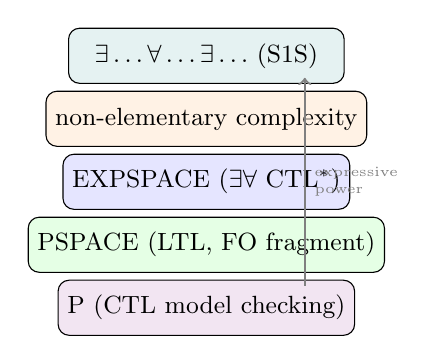
\begin{tikzpicture}[x=2.5cm, y=0.8cm]
    \node[draw, rounded corners, fill=teal!10, font=\small,
          minimum width=3.5cm, minimum height=0.7cm]
          at (0,4) {$\exists\ldots\forall\ldots\exists\ldots$ (S1S)};
    \node[draw, rounded corners, fill=orange!10, font=\small,
          minimum width=3.5cm, minimum height=0.7cm]
          at (0,3) {non-elementary complexity};
    \node[draw, rounded corners, fill=blue!10, font=\small,
          minimum width=3.5cm, minimum height=0.7cm]
          at (0,2) {EXPSPACE ($\exists\forall$ CTL$^*$)};
    \node[draw, rounded corners, fill=green!10, font=\small,
          minimum width=3.5cm, minimum height=0.7cm]
          at (0,1) {PSPACE (LTL, FO fragment)};
    \node[draw, rounded corners, fill=violet!10, font=\small,
          minimum width=3.5cm, minimum height=0.7cm]
          at (0,0) {P (CTL model checking)};
    \draw[->, thick, gray] (0.5, 0.35) -- (0.5, 3.65);
    \node[right, font=\tiny, gray, align=left] at (0.5, 2) {expressive\\power};
  \end{tikzpicture}
  \caption{Complexity vs.\ expressive power in the logic hierarchy.
           Full S1S is non-elementary.  Dropping second-order quantifiers
           gives the FO fragment $\equiv$ LTL $\equiv$ PSPACE.  Dropping
           to CTL (a branching-time restriction) gives polynomial complexity.
           Every step up the ladder gains expressivity at an exponential
           cost.}
  \label{fig:complexity-hierarchy}
\end{figure}

% -----------------------------------------------------------------------
\section{Extensions of S1S}
\label{sec:s1s-extensions}

Over the decades, many extensions of S1S have been studied, some
remaining decidable and some falling into undecidability.
This boundary is pedagogically important: S1S is powerful because it can
quantify over sets of time positions, but its decidability depends on very
specific arithmetic restrictions.

\subsection{S1S over finite words}

\begin{theorem}[Büchi, finite-word version]
A language $L \subseteq A^*$ is \emph{regular} (recognised by some NFA)
if and only if it is \emph{definable in S1S over finite domains}.
\end{theorem}

S1S over finite domains is defined like S1S, but:
\begin{itemize}
  \item The domain is $\{0, 1, \ldots, k\}$ for some $k$ (the length
        of the word minus one), not $\mathbb{N}$.
  \item Second-order variables are interpreted as \emph{finite} sets.
  \item The successor of the last element $k$ is $k$ itself (a self-loop).
\end{itemize}
This gives yet another characterisation of regular languages, alongside
DFA, NFA, and regular expressions.

\subsection{WS1S: Weak Monadic Second-Order Theory}

\begin{definition}[WS1S]
\emph{WS1S} (Weak S1S) is obtained from S1S by requiring that every
second-order variable is interpreted as a \emph{finite} set.
\end{definition}

At first glance this seems much weaker: many of the sets we defined
(all even numbers, all successors of a position, etc.) are infinite
and thus unavailable.  The surprising result is:

\begin{theorem}
WS1S and S1S are \emph{expressively equivalent}: every $\omega$-language
definable in WS1S is also definable in S1S, and vice versa.
\end{theorem}

The non-obvious direction (S1S $\subseteq$ WS1S) is proved via a detour
through \emph{deterministic Muller automata}.  The intuition: although
each set in WS1S is strictly finite, we can simulate infinity by considering a sequence of finite sets of \emph{always increasing size}. The "limit" of these growing finite sets mathematically captures the infinite behavior without ever needing a single infinite set as an object.

\medskip\noindent
\textbf{The fundamental operation.}  The reference operation for Büchi
automata is the \emph{$\omega$-power}: a finite word $u$ followed by
infinitely many copies of some suffix $v$ ($uv^\omega$).  For Muller
automata (which correspond to WS1S), the reference operation is the
\emph{vectorial closure}: infinitely many finite prefixes $v_1 v_2 v_3
\cdots$, each belonging to some set $V$.  This structural difference
reflects the finite-set restriction.

\subsection{Decidable extensions}

Both of the following extensions add a new predicate to S1S:

\begin{description}
  \item[$\mathbf{S1S + P_k}$ (powers of $k$):]
        Add a unary predicate $P_k$ where $P_k(i)$ holds iff $i = k^j$
        for some $j \geq 0$.  For example, $P_2 = \{1, 2, 4, 8, 16,
        \ldots\}$.  The resulting theory is decidable.
  \item[$\mathbf{S1S + \mathrm{Factorial}}$:]
        Add a predicate that holds at positions $1, 2, 6, 24, 120, \ldots$
        ($n!$ for $n \geq 0$).  Still decidable.
\end{description}

\subsection{Undecidable extensions}

\begin{description}
  \item[$\mathbf{S1S + \times 2}$ (doubling function):]
        Add the function $i \mapsto 2i$ (multiply by two).  Decidability
        is lost immediately.  Multiplying by 2 gives enough power to
        simulate arbitrary multiplication, which leads to Peano arithmetic.
  \item[$\mathbf{Peano arithmetic}$ ($\mathbb{N}$ with $+$ and $\times$):]
        Highly undecidable (Gödel incompleteness theorems).
\end{description}

The boundary is surprisingly delicate: adding ``multiply by 2'' destroys
decidability, yet ``powers of $k$'' and ``factorial'' do not.

We now turn from logical expressiveness to a closely related operational
question.  The Büchi theorem says that non-deterministic Büchi automata
capture exactly the S1S-definable languages, but model checking and
synthesis often prefer deterministic monitors, because deterministic
automata are easier to complement and to run inside games.  The next
section is therefore not a second full theory of deterministic
$\omega$-automata.  It is the motivating obstruction that
Chapter~\ref{ch:deterministic-automata-star-free} will resolve with
Muller, Rabin, and parity acceptance.

% -----------------------------------------------------------------------
\section{Deterministic Büchi Automata: Limitations}
\label{sec:dba}

The goal here is intentionally narrow.  We keep the Büchi acceptance
condition and ask whether determinism alone is harmless.  Over finite
words the answer would be yes: every NFA can be determinised.  Over
infinite words the answer is no, and the failure already appears in the
small language of words with finitely many $a$'s.  This witness prepares
the more systematic deterministic theory of
Chapter~\ref{ch:deterministic-automata-star-free}.

\subsection{Definition}

\begin{definition}[Deterministic Büchi Automaton (DBA)]
A \emph{DBA} is a tuple $\mathcal{A} = (Q, A, \delta, q_0, F)$ where
all components are as in an NBA except that $\delta : Q \times A \to Q$
is a \emph{function} (not a relation).  Every state-symbol pair has
exactly one successor.
\end{definition}

\medskip\noindent
\textbf{Operational meaning.}  At runtime, a DBA has no choices to make. Upon reading a symbol, the transition function deterministically forces the automaton into exactly one next state. It completely loses the ability to "guess" future inputs. For a finite word, this isn't a problem, because we can always traverse the whole word and check the end. But for an infinite word, the inability to branch into multiple potential futures and "wait and see" which one becomes successful fundamentally cripples its expressive power.

A DBA has a \emph{unique run} on every $\omega$-word: given $\alpha$,
the run $\sigma = q_0, q_1, q_2, \ldots$ is fully determined by
$q_{i+1} = \delta(q_i, \alpha(i))$.  Acceptance: the unique run is
successful iff $\mathrm{Inf}(\sigma) \cap F \neq \emptyset$.
This uniqueness removes the automaton's ability to ``guess'' a future
event.  That is exactly what will fail in the witness language below.

\subsection{What DBAs can and cannot do}

\begin{proposition}
DBAs are closed under \emph{union} and \emph{intersection}.
\end{proposition}
(Exercise: construct the product automaton and adjust the acceptance condition.)

\begin{theorem}[DBAs are not closed under complementation]
\label{thm:dba-not-complement}
There exists a language $L$ recognised by a DBA such that
$A^\omega \setminus L$ is not recognised by any DBA.  In particular, DBA
languages are not closed under complement and form a \emph{strict subset}
of the $\omega$-regular languages.
\end{theorem}

\subsection{The witness pair: infinitely many vs.\ finitely many \texorpdfstring{$a$}{a}'s}

\begin{definition}
\label{def:Lfin}
Let $A = \{a, b\}$ and:
\[
  L_{\mathrm{fin}} = \{\alpha \in A^\omega \mid
    \alpha \text{ contains finitely many } a\text{'s}\}.
\]
\end{definition}

\begin{proposition}
$L_{\mathrm{fin}}$ is $\omega$-regular.
\end{proposition}
\begin{proof}
A key observation: $\alpha$ contains finitely many $a$'s if and only if
$\alpha$ has a \emph{last $a$}---some final position after which only
$b$'s appear.  The following NBA captures this:

\begin{figure}[ht]
  \centering
  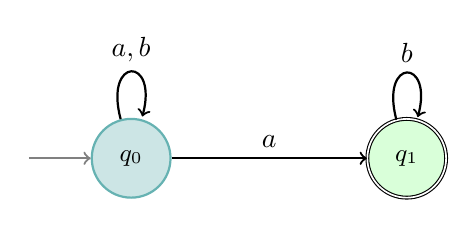
\begin{tikzpicture}[
    st/.style={draw, circle, minimum size=1cm, font=\small},
    acc/.style={draw, circle, minimum size=1cm, font=\small, double},
    arr/.style={->, thick}]
    \node[st, fill=teal!20, draw=teal!60, thick] (q0) at (0,0) {$q_0$};
    \node[acc, fill=green!15] (q1) at (3.5,0) {$q_1$};
    \draw[->, gray, thick] (-1.3,0) -- (q0);
    \draw[arr] (q0) edge[loop above] node[above]{$a, b$} (q0);
    \draw[arr] (q0) -- node[above]{$a$} (q1);
    \draw[arr] (q1) edge[loop above] node[above]{$b$} (q1);
  \end{tikzpicture}
  \caption{NBA for $L_{\mathrm{fin}}$ (finitely many $a$'s).  The
           automaton non-deterministically \emph{guesses} the last
           occurrence of $a$ by taking the transition $q_0 \to q_1$
           and then never seeing $a$ again.}
  \label{fig:nba-lfin}
\end{figure}

\textbf{Why is this correct?}  The automaton ``guesses'' which $a$ is the
last one.  If it guesses correctly (transitions to $q_1$ on the last $a$
and only sees $b$'s thereafter), the run visits $q_1$ infinitely often.
If it guesses wrong (transitions to $q_1$ too early, before the last $a$),
the run gets stuck (no outgoing transition from $q_1$ on $a$).  Since
it is an NBA, the word is accepted iff at least one run is successful.
\end{proof}

\medskip\noindent
\textbf{The complement} $\overline{L_{\mathrm{fin}}}$ = ``infinitely many
$a$'s'' is accepted by the following DBA:

\begin{figure}[ht]
  \centering
  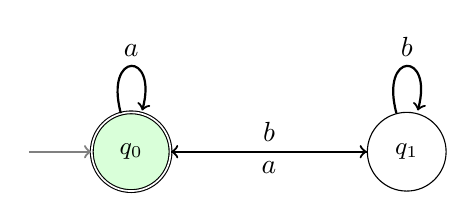
\begin{tikzpicture}[
    st/.style={draw, circle, minimum size=1cm, font=\small},
    acc/.style={draw, circle, minimum size=1cm, font=\small, double, fill=green!15},
    arr/.style={->, thick}]
    \node[acc] (q0) at (0,0) {$q_0$};
    \node[st]  (q1) at (3.5,0) {$q_1$};
    \draw[->, gray, thick] (-1.3,0) -- (q0);
    \draw[arr] (q0) edge[loop above] node[above]{$a$} (q0);
    \draw[arr] (q0) -- node[above]{$b$} (q1);
    \draw[arr] (q1) edge[loop above] node[above]{$b$} (q1);
    \draw[arr] (q1) -- node[below]{$a$} (q0);
  \end{tikzpicture}
  \caption{DBA for $\overline{L_{\mathrm{fin}}}$ (infinitely many $a$'s).
           The accepting state $q_0$ is revisited every time an $a$ is read.
           The word is accepted iff $q_0$ is visited infinitely often,
           i.e., iff there are infinitely many $a$'s.}
  \label{fig:dba-infmany}
\end{figure}

\subsection{Why \texorpdfstring{$L_{\mathrm{fin}}$}{Lfin} has no DBA}

Suppose for contradiction that some DBA $\mathcal{B}$ accepts $L_{\mathrm{fin}}$.
We will construct an infinite word with infinitely many $a$'s that
$\mathcal{B}$ is forced to accept.

Start with a finite prefix $u_0=\varepsilon$.  For any finite prefix $u$,
the word $u b^\omega$ has only finitely many $a$'s, hence belongs to
$L_{\mathrm{fin}}$.  Since $\mathcal{B}$ is assumed to recognise
$L_{\mathrm{fin}}$, the unique run on $u b^\omega$ must visit accepting
states infinitely often.  Therefore, after the prefix $u$, there exists
some number $n$ such that the run reaches an accepting state after reading
$b^n$.

Use this observation inductively.  Having built $u_r$, choose $n_r$ so that
the run reaches an accepting state after $u_r b^{n_r}$, and set
\[
  u_{r+1} = u_r b^{n_r} a.
\]
The limiting word
\[
  \beta = b^{n_0} a\, b^{n_1} a\, b^{n_2} a \cdots
\]
contains infinitely many $a$'s, so $\beta \notin L_{\mathrm{fin}}$.  But the
unique run of $\mathcal{B}$ on $\beta$ visits an accepting state after each
block $b^{n_r}$, hence infinitely often.  Thus $\mathcal{B}$ accepts
$\beta$, a contradiction.

This proves that no DBA recognises $L_{\mathrm{fin}}$.\footnote{A standard
reference for deterministic automata on infinite words is W.~Thomas,
\textit{Automata on Infinite Objects}, in \textit{Handbook of Theoretical
Computer Science}, vol.~B, Elsevier, 1990.}

Theorem~\ref{thm:dba-not-complement} now follows by taking
$L=\overline{L_{\mathrm{fin}}}$, the language ``infinitely many $a$'s'':
Figure~\ref{fig:dba-infmany} gives a DBA for $L$, while the argument above
shows that its complement $L_{\mathrm{fin}}$ has no DBA.

\subsection{Tracing the NBA for \texorpdfstring{$L_{\mathrm{fin}}$}{Lfin} on \texorpdfstring{$abab\cdots$}{ababw}}

\begin{example}[Non-acceptance of $ab^\omega$]
The NBA of Figure~\ref{fig:nba-lfin} should \emph{reject} $abab\cdots =
(ab)^\omega$ (infinitely many $a$'s).  Let us verify:

\begin{center}
\renewcommand{\arraystretch}{1.2}
\begin{tabular}{c|cccccccc}
  Position & 0 & 1 & 2 & 3 & 4 & 5 & 6 & $\cdots$ \\
  \hline
  Symbol   & $a$ & $b$ & $a$ & $b$ & $a$ & $b$ & $a$ & $\cdots$ \\
  \hline
  Run (A): & $q_0$ & $q_0$ & $q_0$ & $q_0$ & $q_0$ & $\cdots$ &  & (not accepting) \\
  Run (B): & $q_0$ & $q_1$ & \textit{stuck} & & & & & (not accepting) \\
\end{tabular}
\end{center}

Run (A) stays in $q_0$ forever (never entering $q_1$): not accepting since
$q_1 \in F$ is never visited.  Run (B) enters $q_1$ after the first $a$
then gets stuck (no transition from $q_1$ on $a$).  Every possible run
either stays in $q_0$ forever or gets stuck---none is accepting.  So
$(ab)^\omega \notin L(\text{NBA})$, as expected.
\end{example}

% -----------------------------------------------------------------------
\section{Towards More Expressive Deterministic Automata}
\label{sec:towards-muller}

The failure of DBAs to accept $L_{\mathrm{fin}}$ shows that determinism
with the Büchi acceptance condition is too weak.  For model checking, we
\emph{need} determinism (to complement specifications efficiently), but we
also need full $\omega$-regular expressiveness.  This is the precise point
at which the chapter hands off to deterministic $\omega$-automata proper:
the proof above is a warning sign, and the repair is to keep determinism
while replacing the acceptance condition.

The solution is to change the acceptance condition.  Two classical approaches:

\begin{description}
  \item[Muller automata:] Accept iff the set of states visited infinitely
        often is exactly one of a specified collection $\mathcal{F}
        \subseteq 2^Q$.  This condition is more refined than Büchi's
        ``at least one state in $F$ infinitely often''.

  \item[Rabin automata:] Accept iff there exists a pair $(E_i, F_i)$ in a
        specified list such that $F_i$ is visited infinitely often
        \emph{and} $E_i$ is visited only finitely often.
\end{description}

Both conditions, when combined with determinism, yield automata equivalent
to NBAs in expressive power---which is exactly what we need.  We will
study these automata and their connection to WS1S in
Chapter~\ref{ch:deterministic-automata-star-free}.

% -----------------------------------------------------------------------
\section{Exercises}
\label{sec:s1s-exercises}

\begin{enumerate}
  \item \textit{(S1S formula writing)}
        Write S1S$_A$ sentences for the following $\omega$-languages over
        $A = \{a, b\}$:
        \begin{enumerate}
          \item $\alpha$ contains \emph{no} $a$'s.
          \item $\alpha$ contains \emph{finitely many} $a$'s.
                (Hint: ``there exists a last $a$''.)
          \item $\alpha$ contains \emph{at least two} $a$'s.
          \item Every $b$ is immediately preceded by an $a$.
        \end{enumerate}

  \item \textit{(Ordering definability)}
        Show that the formula $\varphi(x,y)$ from
        Example~\ref{ex:s1s-order} correctly defines $x < y$ by:
        \begin{enumerate}
          \item Verifying that $\varphi(3, 7)$ is true over $\mathbb{N}$.
          \item Constructing an explicit counterexample set $X$ that refutes
                the \emph{existential} version of the formula when $y = 1$
                and $x = 5$.
        \end{enumerate}

  \item \textit{(Büchi theorem, easy direction)}
        Given the NBA $\mathcal{A}$ with states $Q = \{q_0, q_1\}$,
        initial state $q_0$, $F = \{q_1\}$, and transitions
        $q_0 \xrightarrow{a} q_1$, $q_1 \xrightarrow{b} q_0$,
        write the S1S$_A$ sentence $\Phi_{\mathcal{A}}$ using the
        construction of Section~\ref{sec:buchi-proof-fwd}.
        Identify $\varphi_1$, $\varphi_2$, $\varphi_3$ explicitly.

  \item \textit{(S1S$_0$ translation)}
        Translate the formula $\exists x.\;x \in Q_a \land (x+1) \in Q_b$
        into S1S$_0$ following the four steps of
        Section~\ref{sec:buchi-proof-bwd}.
        Which auxiliary SO variables do you introduce, and why?

  \item \textit{(Base automata)}
        Draw the NBA for $X \subseteq Y$ (Figure~\ref{fig:nba-subset})
        and verify that it accepts the word $(01)^\omega$ but rejects
        $(10)^\omega$.  Verify the run on $00\,(10)\,11^\omega$ and
        determine whether it is accepted.

  \item \textit{(DBA closure)}
        Let $L_1$ and $L_2$ be recognised by DBAs $\mathcal{A}_1$ and
        $\mathcal{A}_2$ respectively.
        \begin{enumerate}
          \item Construct a DBA for $L_1 \cup L_2$.
          \item Construct a DBA for $L_1 \cap L_2$.
          \item Explain why the same product construction does \emph{not}
                work for complementation.
        \end{enumerate}

  \item \textit{(NBA for finitely many A's)}
        Trace the run of the NBA in Figure~\ref{fig:nba-lfin} on the word
        $a b^3 a b^\omega$.
        \begin{enumerate}
          \item List all possible runs.
          \item Identify which runs are accepting.
          \item Conclude whether $ab^3 ab^\omega \in L_{\mathrm{fin}}$.
        \end{enumerate}

  \item \textit{(Non-elementary complexity, intuition)}
        Suppose an S1S formula has exactly 3 quantifier alternations
        (e.g., $\exists\ldots\forall\ldots\exists$) and size $n = 10$.
        Estimate the size of the NBA produced by the Büchi construction
        in the worst case (assume each complementation doubles the number
        of states).  Compare this with $n$, $2^n$, and $\exp(3, n)$.
\end{enumerate}
